\section{Pendule à $N$ maillons}\label{sec:sec3}

\renewcommand*{\overrightarrow}[1]{\vbox{\halign{##\cr 
  \tiny\rightarrowfill\cr\noalign{\nointerlineskip\vskip1pt} 
  $#1\mskip2mu$\cr}}}

Dans cette partie, nous considérons le pendule simple et double, et nous cherchons à
résoudre leurs équations de mouvement par les méthodes numériques implémentées en section~\ref{sec:sec1}.

\subsection{Pendule simple}
Dans le cas du pendule simple, deux forces s'appliquent sur la masse $m$:
le poids de la masse \overrightarrow{P} et la force de la tige \overrightarrow{T}.
Selon le théorème du moment cinétique appliqué en $M$ par rapport à $O$, on a
$\frac{d\overrightarrow{L_{O,M}}}{dt} = \overrightarrow{M_{O, M}(\overrightarrow{P})} + \overrightarrow{M_{O, M}(\overrightarrow{T})}$.
Or, le moment de \overrightarrow{T} est nul, car \overrightarrow{OM} et \overrightarrow{T} sont colinéaires.
En développant, on obtient $m l^{2} \ddot \theta = - m l g \sin{\theta} $, ce qui nous donne finalement $\ddot \theta + \frac{g}{l} \sin{\theta}= 0$.

On retrouve l'équation différentielle non-linéaire du second ordre bien connue du pendule simple. 
Pour la résoudre numériquement en fonction de l'angle initial $ \theta_0 $, et de la vitesse initiale $ \dot \theta_0 $,
on peut utiliser une des méthodes implémentées auparavant, comme par exemple la méthode d'Euler.
Une fois que la fonction $ \theta(t) $ a été approchée, on peut calculer la période du pendule en prenant la différence entre 
deux maxima successifs, ce qui permet de déterminer la fréquence.

En affichant les fréquences du pendule pour $ \theta_0 $ variant de $ -\frac{\pi}{2} $ à $ \frac{\pi}{2} $, 
on obtient la figure~\ref{fig:frequences}.
La fréquence pour de petites oscillations, $ \frac{1}{2 \pi} \sqrt{\frac{g}{l}} $, semble respectée.

\begin{figure}[htbp!]
	\centering
	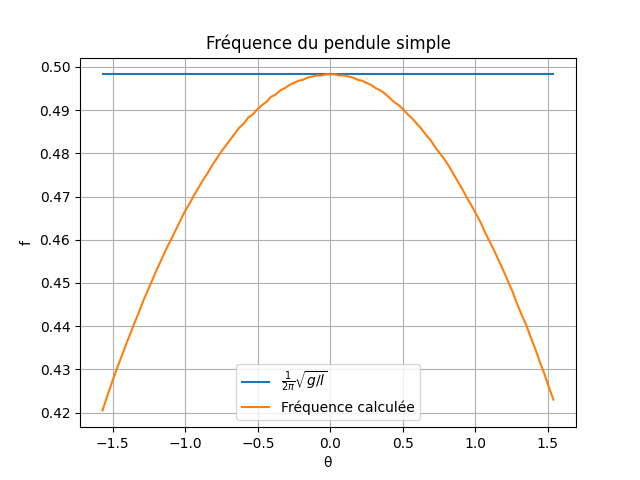
\includegraphics[width=0.42\textwidth]{res/freq_pendule_simple.png}
	\caption{Fréquence du pendule en fonction de l'angle initial $ \theta_{0}$}
	\label{fig:frequences}
\end{figure}


\subsection{Double pendule}

Le pendule à deux maillons est constitué de deux masses $ m_1 $ et $ m_2 $ 
reliées par deux tiges de longueur $ l_1 $ et $ l _2 $. On note $ \theta_1 $ et $ \theta_2 $ les angles
que font les tiges avec la verticale. Dans la littérature, on trouve les deux équations donnant $\ddot \theta_1$ et $\ddot \theta_2$ en fonction des autres paramètres.

La mise sous forme du système d'équations différentielles comme précisé en première partie est plus complexe,
puisqu'il faut passer par un vecteur de résolution de dimension $4$.
En effet, le système possède $4$ conditions initiales, à savoir les angles initiaux, et les vitesses initiales.
On a donc le vecteur $ U = (\theta_1, \theta_2, \dot \theta_1, \dot \theta_2) $, et on peut donc écrire sa dérivée en fonction de ses variables, et des équations donnant $\ddot \theta_1$ et $\ddot \theta_2$,
ce qui nous donne le vecteur $ U' = (\dot \theta_1, \dot \theta_2, \ddot \theta_1, \ddot \theta_2) $.

Contrairement au pendule simple, le pendule double admet une trajectoire qui est très sensible aux conditions initiales, par son caractère chaotique, comme le montre la figure~\ref{fig:retournement}.

Une fois les trajectoires calculées, on peut s'intéresser au temps que met le pendule à se retourner (la masse $ m_2 $ passe au-dessus de $ m_1 $).
Ce retournement arrive lorsque $ \theta_2 $ dépasse en valeur absolue $ \pi $.
Pour des valeurs faibles des conditions initiales, le pendule ne se retourne pas, comme dans la figure~\ref{fig:no_retournement},
où $ \dot \theta_2 = 4 $ rad/s, et les autres conditions initiales sont nulles.
En revanche, lorsqu'on augmente les vitesses angulaires, on observe généralement un retournement du pendule, comme dans la figure~\ref{fig:retournement}.

\begin{figure} [H]
	\begin{minipage}[c]{0.4\textwidth}
		\centering
		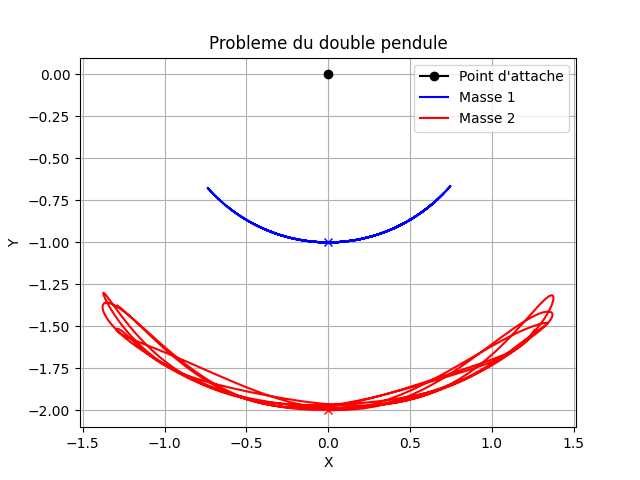
\includegraphics[width=\textwidth]{res/no_retournement.png}
		\caption{$\dot \theta_2 = 4$ rad/s.}
		\label{fig:no_retournement}
	\end{minipage}\hfill
	\begin{minipage}[c]{0.4\textwidth}
		\centering
		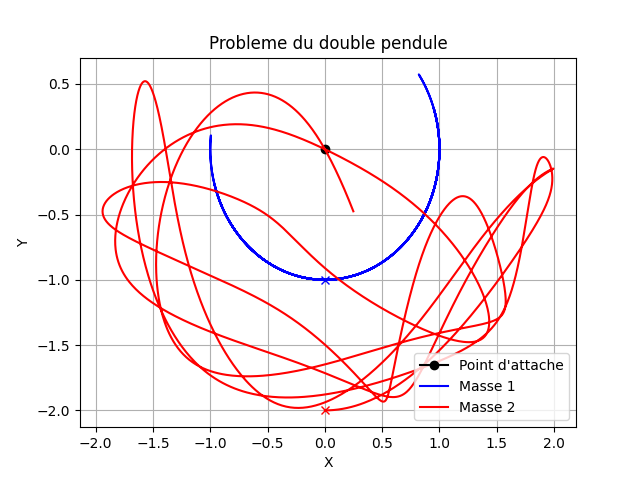
\includegraphics[width=\textwidth]{res/retournement.png}
		\caption{$\dot \theta_2 = 8$ rad/s.}
		\label{fig:retournement}
	\end{minipage}
\end{figure}
